%!TEX root = /Users/domaubert/Documents/Lectures/cosmologie/cosmo_main.tex
\chapter{Entropie et Univers}
\newthought{La notion d'entropie est profondément liée}\index{entropie} à la cosmologie. En thermodynamique classique, l'entropie est la quantité centrale liée au \textit{second principe}\index{second principe de la thermodynamique} qui stipule que toute transformation d'un système physique s'accompagne d'une création d'entropie $S$\sidenote{notée ainsi en hommage à Sadi Carnot}:
\begin{equation}
\Delta S \ge 0
\end{equation}
Au mieux, l'entropie reste constante dans le cas d'une transformation dite réversible mais dans tous les cas elle ne peut diminuer : si cela est malgré tout constaté, cela signifie qu'il existe un autre système, en contact avec celui étudié, qui voit son entropie augmenter d'au moins d'autant que la diminution\sidenote{avec $\Delta S_1<0$ et $\Delta S_1 +\Delta S_2>0$} 

L'une des découvertes fondamentales de la cosmologie est l'affirmation que notre Univers évolue et possède donc une histoire. Conformément à sa définition, cela implique que l'entropie de l'Univers fut plus basse dans le passé qu'elle n'est aujourd'hui. Par ailleurs, l'Univers possède clairement une capacité d'évolution future et son entropie est donc amenée à augmenter. Nous sommes donc aujourd'hui dans un niveau d'entropie intermédiaire, ni à son niveau le plus bas ni à son niveau le plus élevé et cela pose donc naturellement question.

\section{Configurations et probabilités}
\newthought{L'entropie est une mesure} du nombre d'états microscopiques\index{etats@états microscopique} correspondant à un état macroscopique donné. Dans l'ensemble micro-canonique\index{micro-canonique}, décrivant des systèmes isolés à énergie constante, cette brève définition est rigoureusement exacte. L'entropie micro-canonique $S$ est donnée par:
\begin{equation}
S=k_B\log \Omega
\end{equation}
où $\Omega$ désigne le nombre de configurations correspondants à un état macroscopique donné. Le second principe de la thermodynamique\index{second principe} stipule que tout système isolé tend à voir son entropie augmenter avec le temps, au pire elle stagnera si le système atteint un état d'équilibre. Par extension, la flèche du temps\index{flèche du temps} est régie par le sens d'évolution de l'entropie : si 2 possibilités s'offrent à un système, l'une avec une augmentation de l'entropie, l'autre avec une diminution de celle-ci, c'est la première qui sera privilégiée.

Cette croissance imposée à l'entropie peut paraître ad hoc, mais émerge naturellement quand on considère l'entropie micro-canonique. Prenons par exemple un système composé de 4 particules avec 2 éléments gris et 2 éléments rouges (cf. Figure \ref{f:micro}) : ce système peut être \textit{ordonné}\sidenote{ordonné désigne dans notre un exemple un état où les couleurs sont séparées}, un état macroscopique atteint par 2 configurations différentes, ou bien \textit{désordonné}, un autre état macroscopique atteint lui par 4 configurations différentes. Dans l'ensemble micro-canonique, chacune de ces 6 configurations est équiprobable et étant dans une certaine configuration de départ, notre système peut passer dans n'importe quelle autre avec une égale probabilité. Par contre ce raisonnement ne tient pas lorsqu'on considère les états macroscopiques.
En particulier, si le système est dans un état ordonné, il a dans ce cas 2 fois plus de chances d'évoluer vers un état désordonné que de rester ordonné.  A l'inverse, si il se trouve dans un état désordonné, il a deux fois plus de chances de rester désordonné.
\begin{figure}[htbp]
	\centering
		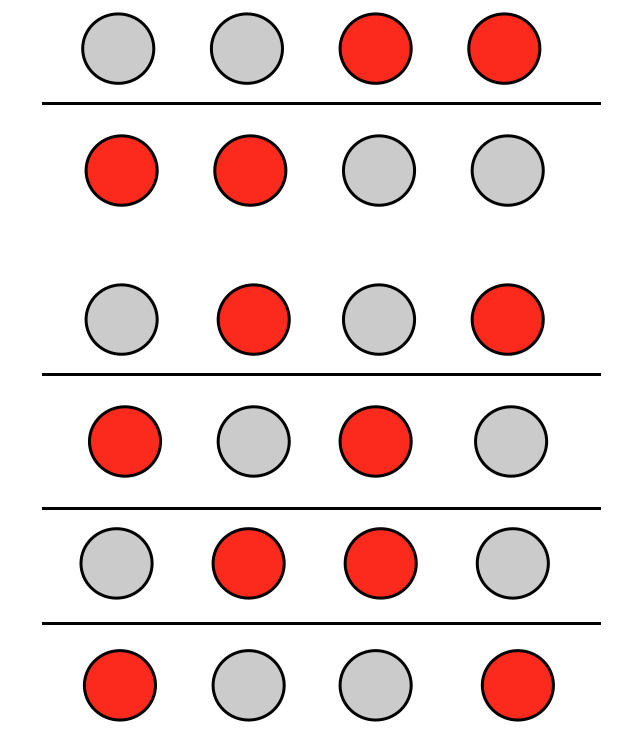
\includegraphics[height=7cm]{figs/micro.png}
	\caption[micro-états disponibles dans un système simple comprenant 2 paires de boules de couleurs identiques]{Tous les micro-états disponibles dans un système simple comprenant 2 paires de boules de couleurs identiques. On note que le macro-état 'couleurs séparées' est moins probables que le macro-état 'couleurs mélangées'.}
	\label{f:micro}
\end{figure}

\newthought{Il n'y a pas de magie noire} : le système évolue vers l'état qui a le plus de chance d'être réalisé. Dans notre cas, l'état mélangé est plus probable que l'état rangé. A l'inverse, l'état rangé est mieux \textit{connu} que l'état mélangé : si le système est dans l'état rangé et que l'on s'interroge sur la 'vraie' configuration sous-jacente, on ne peut guère se tromper car il n'en existe que 2. A l'inverse si le système est dans l'état mélangé, la probabilité de deviner la configuration exacte sous-jacente est 2 fois plus faible : globalement nous avons une meilleure connaissance de la configuration\index{entropie!configuration} exacte du système si il est dans un état de faible entropie. C'est pour cette raison que l'entropie est également une mesure du niveau d'information\index{entropie!information} ou de méconnaissance que nous avons du système : un système avec une entropie élevée est moins bien connu qu'un système à basse entropie et cette connaissance à tendance à se dégrader avec le temps. C'est la contrepartie d'une évolution qui va naturellement vers les états à grands nombre de configurations.

Ces constatations restent applicables pour des systèmes plus complexes ou plus réalistes. Par exemple, le nombre de configurations correspondant à un verre brisé excède de très loin celui correspondant à un verre intact : ce dernier nécessite un arrangement précis des atomes et tout départ léger à cet arrangement conduit à le casser. Par conséquent, l'évolution naturelle d'un verre est d'évoluer vers un état cassé, de plus grande entropie. De même si l'on veut recoller un verre (et donc baisser son entropie), cela est quasi-impossible si celui-ci est isolé : il faudrait que spontanément les atomes trouvent l'unique configuration qui corresponde au verre intact parmi toutes celles qui sont associées à un verre brisé. Reconstituer le verre nécessite d'ouvrir le système afin que la baisse d'entropie du verre soit compensée par une augmentation plus globale de l'entropie \sidenote{Par exemple, pour recoller un verre il faut qu'un individu s'attelle à cette tâche. La réflexion de cet individu va nécessairement produire de la chaleur, chaleur qui va globalement augmenter l'entropie}. 

\newthought{La témpérature et l'entropie}\index{température!entropie} sont souvent associées et à nouveau on retrouve dans cette association la notion d'ordre et de désordre, d'information et de méconnaissance. Pour un gaz parfait confiné dans une enceinte, la température est liée à la dispersion de vitesses des particules le composant : on peut montrer que celle ci est de l'ordre de
\begin{equation}
\sigma \sim \srqt{k_B T}
\end{equation}
et la distribution de vitesse\index{vitesse!distribution} des particules suit une loi normale\sidenote{type distribution de Maxwell-Boltzmann} d'écart-type donné par cette dispersion (voir Fig. \ref{f:disp}). Si le gaz possède une température élevée, la dispersion de vitesse est importante et par conséquent le spectre des valeurs de vitesses atteignables par une particule est très étendu. A l'inverse, un gaz froid implique une gamme de vitesses accessibles beaucoup plus contrainte.
\begin{figure}[htbp]
	\centering
		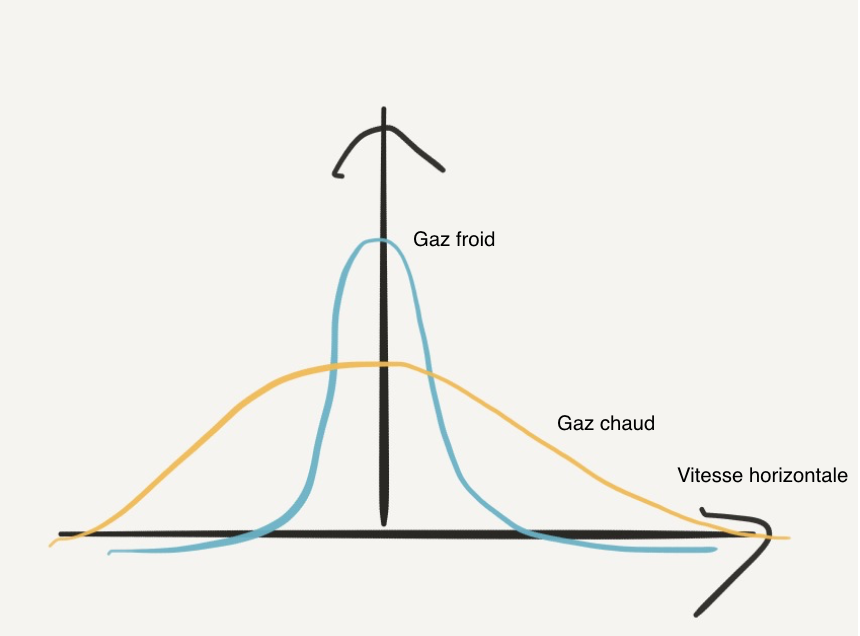
\includegraphics[height=7cm]{figs/dispersion.png}
	\caption[Le lien entre la dispersion de vitesse et la température du gaz. ]{Le lien entre la dispersion de vitesse et la température du gaz. En général la distribution des vitesses suit une courbe gaussienne, centrée en zéro (la particule n'a pas choisi si elle va à gauche ou à droite) avec des ailes décroissantes. La température est une mesure de la largeur de la distribution: une grande température est la marque de particules à très grande vitesse.}
	\label{f:disp}
\end{figure}
Si on considère que ces gaz chauds et froids sont dans la même cuve (donc dans un volume donné), la portion d'espace des vitesses accessible au gaz chaud est plus grande que celle accessible au froid : le nombre d 'états correspondant à un gaz chaud est plus important que celui du gaz froid et possède donc une plus grande entropie. Prenant le point de vue inverse, il est plus difficile de prédire la vitesse d'une particule du gaz chaud que pour celle d'un gaz froid. 

Par ailleurs, on dispose d'un certain niveau d'information sur ce mélange : si on prend au hasard une particule et que l'on mesure sa vitesse comme étant élevée, on peut sans trop se tromper l'associer au gaz chaud et à l'inverse si sa vitesse est faible, il y a de plus grandes chances qu'elle appartienne au gaz froid. Par conséquent l'évolution naturelle du système est vers une plus grande méconnaissance, vers la thermalisation\index{thermalisation} des deux gaz vers une même température, intermédiaire entre les 2 températures initiales où le mélange devient tiède. Dans ce cas là, il y a une perte d'information : la mesure de la vitesse ne permet plus de distinguer les 2 gaz originaux. C'est aussi pour cela que les 2 gaz n'évoluent pas vers une plus grande différence de température, le froid devenant encore plus froid et le chaud encore plus chaud : cela augmenterait notre capacité à distinguer les 2 gaz en tirant les particules au hasard, en contradiction avec la dégradation de l'information posée par le second principe.

\section{Entropie et perception du temps}

\newthought{L'entropie augmente} irrémédiablement lorsqu'un système évolue de manière isolée, toutefois cette augmentation peut ralentir voir s'arrêter. Dans ce dernier cas, le système a atteint un état stationnaire ou d'équilibre\index{etat@état d'équilibre} : cet état macroscopique est le plus probable parmi tous les possibles et possède donc la plus grande chance d'être sélectionné parmi tous ceux accessibles. Un exemple est donné dans la figure \ref{f:equi}. La configuration initiale correspond à un gaz confiné à un sous-volume d'une cuve plus grande : l'évolution naturelle du système va amener le gaz à s'étendre et occuper la cuve dans sa totalité. En supposant que la température du gaz n'évolue pas (et donc que le spectre des vitesses atteignables par les particules reste inchangé), la configuration "cuve remplie" fournit davantage de configurations possibles que lorsque que le gaz est confiné dans une sous-partie : dit simplement le nombre de positions accessibles est plus important lorsque le gaz est étendu. L'entropie de la configuration finale est plus importante que celle de départ. 
\begin{figure}[htbp]
	\centering
		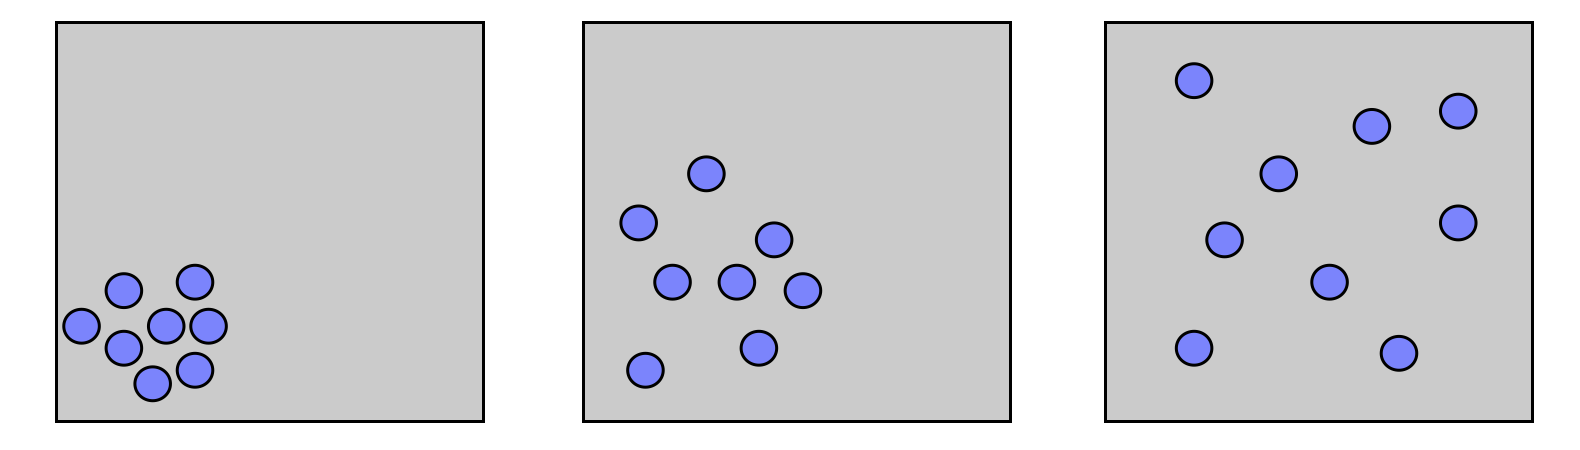
\includegraphics[height=5cm]{figs/equiconfig.png}
		%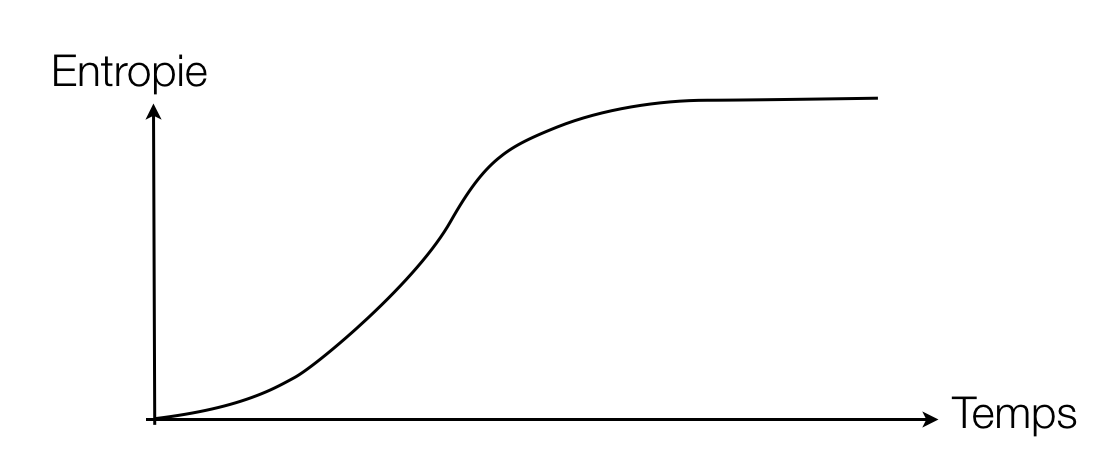
\includegraphics[height=5cm]{figs/equientro.png}
\caption[Remplissage d'une cuve par un gaz]{Le gaz initialement confiné en bas à gauche remplit peu à peu la cuve. La dernière situation a une entropie plus importante que la première car le nombre de positions accessibles aux particules est plus important. Par contre arrivé à ce stade, l'entropie ne peut plus augmenter de façon significative, on a donc un maximum d'entropie.}
	\label{f:equi}
\end{figure}

Une fois la cuve remplie, le système ne peut cependant plus évoluer et cela correspond à une maximisation des configurations atteignables: le système a atteint un maximum d'entropie\index{entropie!maximum}. Une représentation schématique de l'évolution temporelle de l'entropie est donnée en figure \ref{f:equitemps} : au delà d'une durée caractéristique \sidenote{intuitivement cette durée $t^*$est liée à la taille de la cuve $L$ et à la vitesse caractéristique $\sigma \sim\sqrt{k_B T}$.  Avec $t^*\sim L/\sqrt{T}$, on constate que l'équilibre est d'autant plus rapidement atteint que la température est élevée.}, $S(t)$ atteint un plateau, autour duquel la valeur peut éventuellement fluctuer mais jamais redescendre. A ce stade, on constate que le temps est une mauvaise mesure de l'évolution du système: le temps continue à changer sans que le système n'évolue. A l'inverse, l'entropie donne une meilleure représentation de la réalité physique du gaz : l'entropie stagne de la même manière que le système n'évolue plus. Un observateur regardant ce système qui n'évolue plus pourra légitimement dire que le temps a gelé ou bien que le temps est long, car plus rien ne se passe. Par rapport à ce vécu empirique, il apparaît clairement que l'entropie joue un meilleur rôle de représentation de l'évolution du monde : elle augmente lorsque les choses changent, elle stagne lorsque le monde se fige. 
\begin{figure}[htbp]
	\centering
		%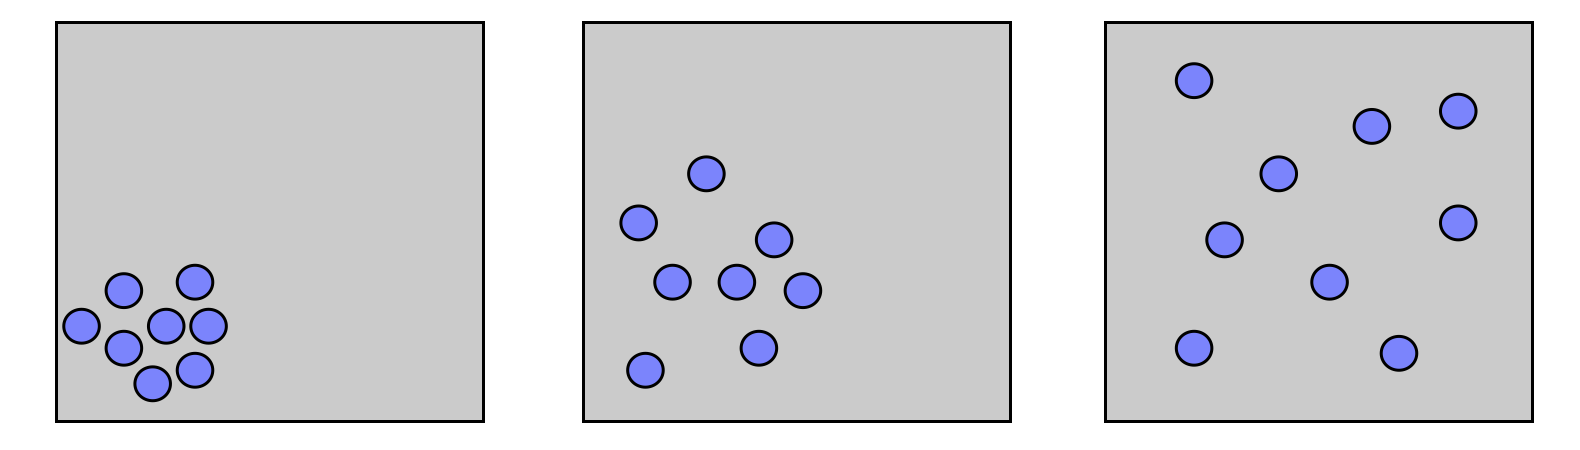
\includegraphics[height=5cm]{figs/equiconfig.png}
		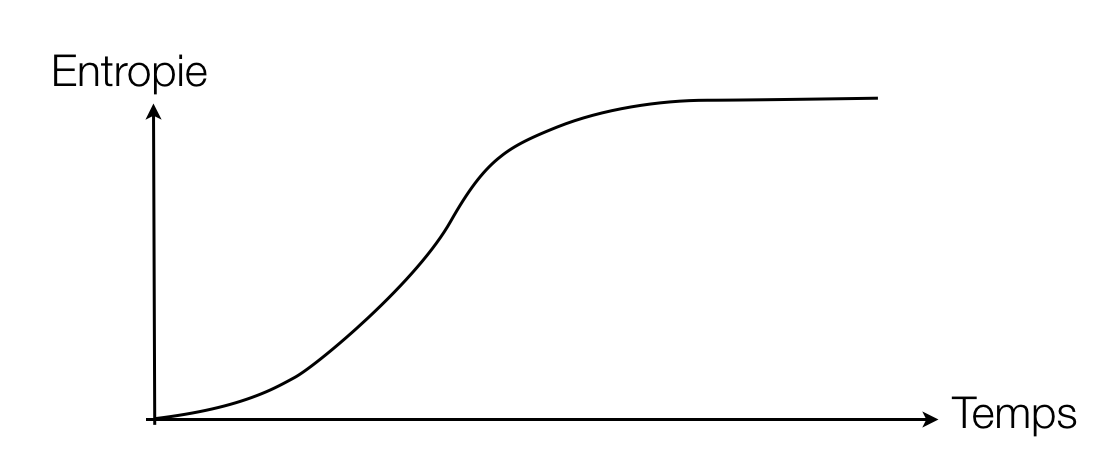
\includegraphics[height=5cm]{figs/equientro.png}
	\caption[Evolution vers un maximum d'entropie]{Un système peut accéder à un maximum d'entropie, auquel cas il n'évolue plus. Le temps est long, car l'entropie est quasi-constante. A l'inverse la phase où l'entropie varie rapidement traduit un système en évolution rapide, durant laquelle le temps s'écoule rapidement.}
	\label{f:equitemps}
\end{figure}

\newthought{Le temps possède une double nature}: c'est d'une part une coordonnée, qui nous permet de nous repérer dans l'espace-temps et une mesure de 'distance' qui permet de quantifier le parcours ou le voyage réalisé par un système au cours du temps. Ces deux concepts ne sont pas nécessairement interchangeables et il s'avère que l'on peut se déplacer sans voyager. Par exemple, le voyageur peut arguer du fait qu'un alpiniste ne voyage pas et que son déplacement vertical, tout important qu'il soit sur les plus hauts sommets himalayens par exemple, ne lui permet pas de voir du monde : déplacement et voyage ne vont pas forcément de paire. Le temps et l'entropie\index{temps!entropie} ont le même type de relation : dans une vision entropique le temps c'est du changement et dans une certaine mesure c'est une définition qui est proche de notre vécu empirique. Lorsqu'il ne se passe rien, le temps s'écoule pas ou peu\sidenote{on dit aussi que l'\textit{on trouve le temps long}}. Dans ce régime le temps du chronomètre $t$, celui qui s'écoule inexorablement, est une piètre mesure de la réalité vécue et dans certaines circonstances on aimerait que le temps passe plus vite : dans ces circonstances, c'est réellement $S$ qui est invoqué, et non pas $t$. A l'inverse lorsque les systèmes évoluent rapidement, le temps s'écoule rapidement \sidenote{on dit aussi que l'on trouve que \textit{le temps passe vite}}. Parfois on aimerait plus de temps ou bien l'on explique que le temps passe trop vite : à nouveau ce n'est pas le temps $t$ du chronomètre qui est évoqué ici, mais bien l'entropie $S$ dont on  aimerait qu'elle évolue plus lentement.

\section{Entropie et Complexité}
\newthought{On confond souvent entropie et complexité}\index{entropie!complexité}. L'entropie est une mesure du nombre de configurations correspondant à un état macroscopique donné tandis que la complexité est une mesure du nombre d'informations\index{information} qu'il faut pour décrire l'état d'un système. La figure \ref{f:melange} illustre la différence entre ces 2 concepts: on y voit le mélange progressif de 2 gaz, l'un bleu l'autre jaune pour aboutir in fine à un ensemble de couleur verte. Comme vu précédemment, cette évolution implique nécessairement une augmentation de l'entropie : la situation initiale confine chacun des gaz dans un sous-volume et chaque particule dispose d'un ensemble de configurations spatiales limité. Par ailleurs, l'observateur a une bonne connaissance du système: une particule jaune est nécessairement à droite, une bleue nécessairement à gauche. Lorsque le mélange procède, la connaissance de l'état du système se dégrade peu à peu : chaque particule a désormais accès à une plus grande portion du volume et dans l'état final, les 2 fluides disposent de tout le volume pour s'étendre et donc d'un grand nombre de configurations. Par ailleurs on constate à nouveau une dégradation de l'information puisqu'il est impossible de lier couleur et position.
\begin{figure}[htbp]
	\centering
		%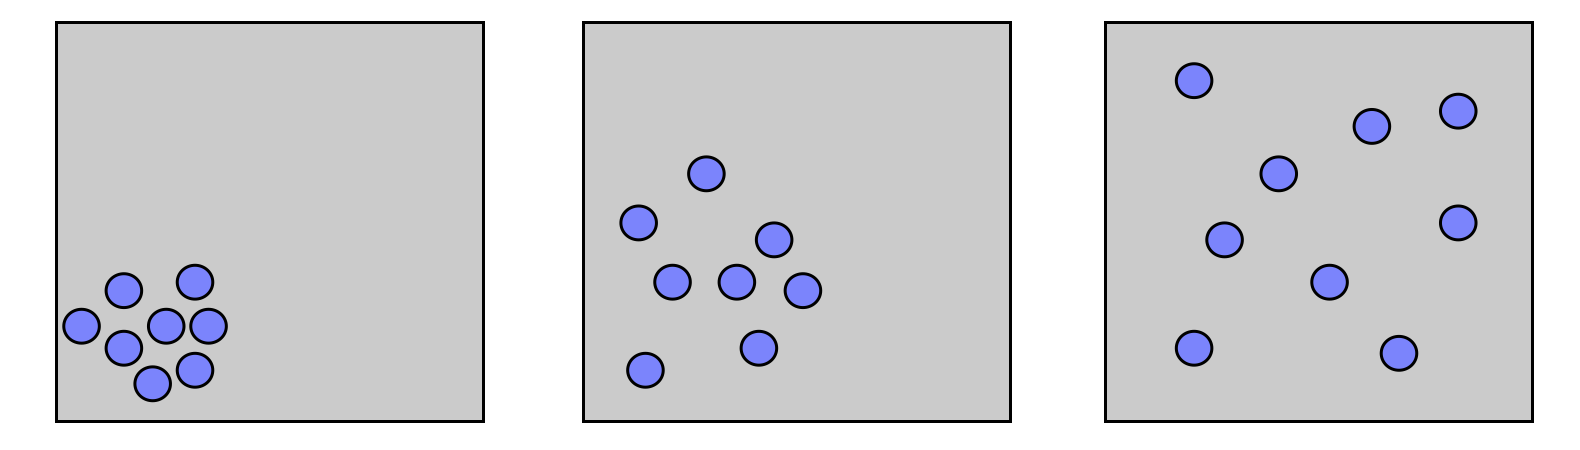
\includegraphics[height=5cm]{figs/equiconfig.png}
		
\includegraphics[height=5cm]{figs/melange.png}
		\caption[Entropie \& Complexité]{Réprésentation schématique du mélange de 2 gaz. L'entropie va augmenter de gauche à droite tandis que la complexité va passer par un maximum, correspondant à l'état intermédiaire. La présence d'une interface complexe, rend la complexité globale de cette étape très importante. La dernière situation est simple (peu complexe à décrire) mais par contre son entropie est maximale.}
	\label{f:melange}
\end{figure}

La complexité évolue différemment et n'évolue généralement pas de manière monotone. Dans l'exemple précédent, les états initiaux et finaux sont globalement 'simples' : l'état macroscopique initial est simple à décrire puisque la position permet de définir la couleur des particules tandis que l'état final l'est encore plus du fait de son homogénéité. L'état intermédiaire en revanche est bien plus difficile à décrire à cause de la zone de mélange : cette zone requiert que l'on établisse un certain nombre de paramètres pour pouvoir être reproduite. Pour cet exemple, la complexité passe par un maximum avant de décroître: l'augmentation de l'entropie nécessite de passer par un pic de complexité. Ce passage par une complexité maximum est souvent la route la plus efficace pour une augmentation de l'entropie. Par exemple la transformation d'une matière première en chaleur passe souvent par l'intermédiaire d'une 'machine' complexe, comme un animal pour de la nourriture ou un moteur pour du carburant.

{Désorganisation et complexité} sont 2 choses différentes : un système peut être dans un état très désorganisé ou peu contraint sans que sa complexité soit grande. C'est le cas de l'état final de l'exemple de la figure \ref{f:melange} : il est simple à décrire mais pour autant un observateur sait très peu de choses dessus. Sa complexité est faible mais son entropie est élevée. 

\section{Entropie et formation des grandes structures}
\newthought{Les liens entre cosmologie et entropie} sont nombreux et posent parfois problème. Le plus fameux d'entre eux est l'impression que l'Univers s'organise au cours du temps : durant les premiers instants, le cosmos est par exemple peu structuré et la marche du temps s'accompagne de la mise en place d'objets de plus en plus complexes tels que les étoiles\index{etoiles@étoiles}, les galaxies\index{galaxies} et les amas. Le mécanisme d'instabilité gravitationnelle\sidenote{étudiée en détail dans la section dédiée, page \pageref{s:struct}} donne ainsi l'apparence d'une organisation croissante des objets en contradiction apparente avec le second principe de la thermodynamique. 

Cette contradiction n'est bien sûr qu'apparente et peut être levée de plusieurs façons. Par exemple, on peut aisément invoquer le fait que le processus qui va transformer un nuage de gaz en galaxie n'est pas gratuit. Comme vu précédemment, une galaxie ne peut se mettre en place que si elle parvient à atteindre des densités très élevées \sidenote{typiquement plusieurs milliers de fois la densité moyenne globale}. Or l'énergie interne du gaz (liée à sa pression) s'oppose à ce que de telles densités soient atteintes et ce la n'est possible qu'en évacuant cette énergie hors du gaz : dans l'Univers cette évacuation opère via des processus atomiques ou moléculaires qui convertissent l'énergie cinétique microscopique en rayonnement. Ce rayonnement\index{entropie!rayonnement} emporte cette énergie et permet d'atteindre les densités à même de mettre en place des galaxies ou de la formation stellaire en leur sein. Ce processus est producteur d'entropie : des particules (atomes/molécules) en génèrent d'autres, les photons\index{photons}, et parfois en grand nombre. Cette évacuation d'énergie\sidenote{voir le chapitre dédié à la formation des petites structures}, que l'on désigne également par le terme de \textit{refroidissement}\index{refroidissement}, fait grandir le nombre de configuration possible accessible par le système par simple production de particules : en augmentant leur nombre, le système augmente le nombre de degrés de libertés et donc son entropie. Par ailleurs les photons occupent naturellement un grand volume, augmentant d'autant le nombre de configurations possibles pour un état macroscopique donné.  Pour s'organiser, un sous-ensemble de particules (les atomes) vont désorganiser l'ensemble en produisant un grand nombre de particules supplémentaires (le rayonnement).

Mentionnons toutefois que ce type de mécanisme où l'entropie est générée en évacuant l'énergie vers l'extérieur n'est pas limitée à des processus baryoniques. Pour des systèmes stellaires comme les amas globulaires\index{amas globulaire}, où les constituants n'interagissent que via la gravitation, on trouve également des processus similaires comme la \textit{catastrophe gravothermale}\index{catastrophe gravo-thermale}. Cette dernière consiste en l'effondrement d'un coeur associé à l'expansion d'une enveloppe dans un système non-collisionnel. Dans ce processus l'énergie gravitationnelle libérée par l'effondrement interne va profiter aux couches externes et générer de l'entropie. De même lors de la viriélisation d'un halo\index{halo}, l'effondrement sphérique\index{effondrement sphérique} va 'thermaliser' et redistribuer les orbites des particules de matière noire : initialement toutes ces orbites sont radiales (forte information sur la dynamique, faible entropie) et vont évoluer en un comportement beaucoup plus thermique et désordonné (donc difficile à connaître, forte entropie) après la mise à l'équilibre.

En résumé la complexité croissante des structures apparaît de prime abord comme en contradiction avec le 2nd principe : toutefois, cette complexité s'accompagne dans tous les cas d'une production d'entropie. De plus cette complexité ne peut devenir arbitrairement grande : les petites étoiles s'arrêtent et refroidissent, l'expansion accélérée\index{expansion!accélération} créée par la constante cosmologique va supprimer les interactions entre galaxies, les planètes vont cesser de produire de la chaleur\sidenote{cette production est régie par la présence d'éléments radioactifs qui finissent par s'épuiser, cf. Venus ou Mars qui ne possèdent plus d'activité interne.}, etc... ~: ces quelques exemples sont autant d'illustration de la \textit{mort thermique}\index{entropie!mort thermique} qui attend l'Univers. Cette mort thermique désigne cet état futur où l'entropie ne sera plus en mesure de croître indéfiniment, conduisant de fait à un état d'équilibre de l'Univers. Dans cet Univers, il ne se passe plus rien, l'entropie stagne.

\section{Le défi de l'entropie actuelle}

\newthought{L'entropie actuelle de l'Univers est basse}. Par définition, elle fut encore plus basse dans le passé mais comparée à ce qu'elle pourrait être, l'entropie actuelle de l'Univers se trouve à de très faibles niveaux\index{entropie!initiale}\sidenote{on peut évaluer l'entropie maximale atteignable par l'Univers et mettant tout son contenu dans un trou noir. L'information ne sort pas de l'objet, la méconnaissance et donc l'entropie est maximale. On en est très loin.}. Par conséquent le potentiel d'évolution de l'Univers est grand et se pose naturellement la question \textit{pourquoi l'entropie actuelle est-elle si basse ?} En effet, imaginons que l'Univers que nous connaissons soit le fruit d'un tirage de lois, paramètres physiques, géométries, etc... parmi tous les ensembles disponibles : normalement, un tel tirage doit naturellement tomber sur les états macroscopiques les plus représentés, les plus probables, donc ceux avec l'entropie la plus forte possible. Dit autrement l'Univers aurait eu toutes les raisons d'avoir une capacité d'évolution faible, avec une entropie élevée, si il avait été choisi par hasard ce qui est la définition même de la \textit{perfection}\index{perfection} à savoir un système \textit{qui n'a pas besoin de changer}. Or ce n'est pas le cas, notre Univers n'est pas parfait.

Ce genre de questionnement amène généralement 2 types de réponses~: l'entropie est basse du fait d'un mécanisme ou du fait de conditions initiales. Si c'est le fait de conditions initiales, la question est close et le potentiel d'évolution de notre Univers fait partie de ses propriétés intrinsèques au même titre par exemple que les paramètres cosmologiques. Bien que possible, cette hypothèse nous intéresse peu et la tentation est grande d'essayer de trouver un mécanisme qui produit naturellement une entropie basse aux premiers instants.

Il existe un mécanisme simple et non exotique qui permette d'expliquer une entropie initiale basse : ce mécanisme repose sur la nature statistique des quantités macroscopiques. Lorsque qu'un système évolue son entropie augmente: cette affirmation doit s'entendre de façon statistique. L'entropie est une quantité qui est définie de façon statistique\index{entropie!fluctuation} via par exemple sa valeur moyenne ou son écart-type : sa valeur moyennée sur une certaine durée va augmenter inexorablement dans un système en évolution tout en fluctuant sur des échelles de temps plus courtes. A un instant donné, un système peut voir son entropie baisser ponctuellement avant de reprendre sa croissance\sidenote{nous l'avons vu dans notre exemple simple à base de boules colorées : il est possible de retourner à une situation où les couleurs sont séparées, même si cela est mois probable que de rester dans une situation désordonnée}. On peut imaginer que l'entropie basse de l'Univers fut généré par ce type de fluctuations\index{fluctuation d'entropie} : l'Univers aurait été dans un état de 'pseudo-équilibre' avec une entropie constante sur des temps longs et une fluctuation accidentelle et suffisamment grande aurait octroyé à notre Univers un potentiel d'évolution.
\begin{figure}[htbp]
	\centering
		%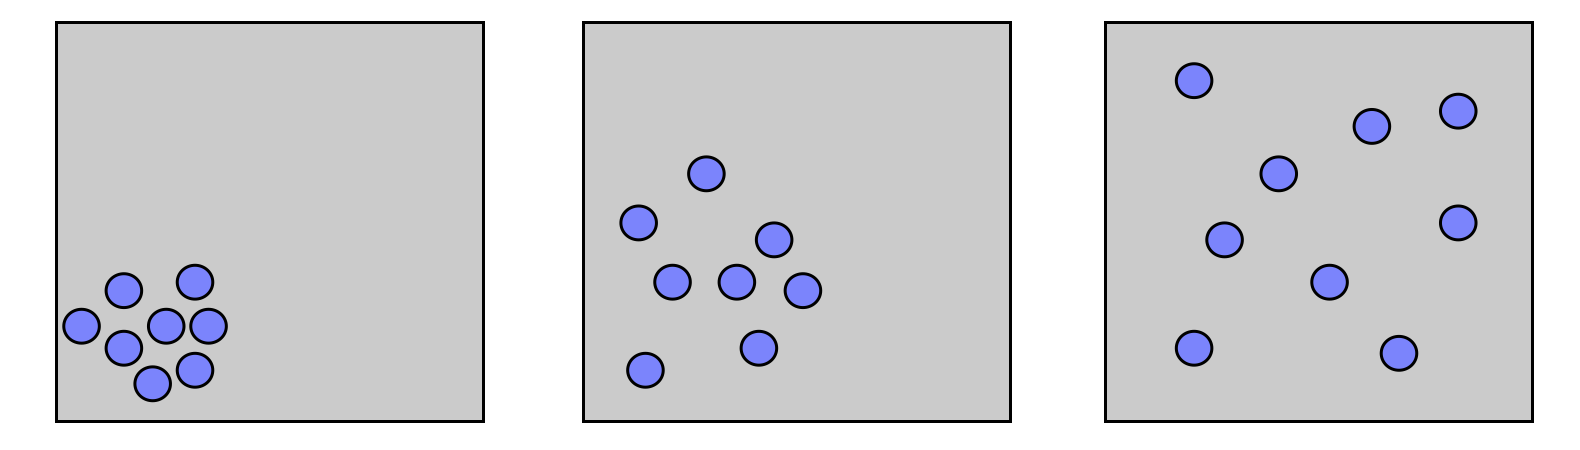
\includegraphics[height=5cm]{figs/equiconfig.png}
		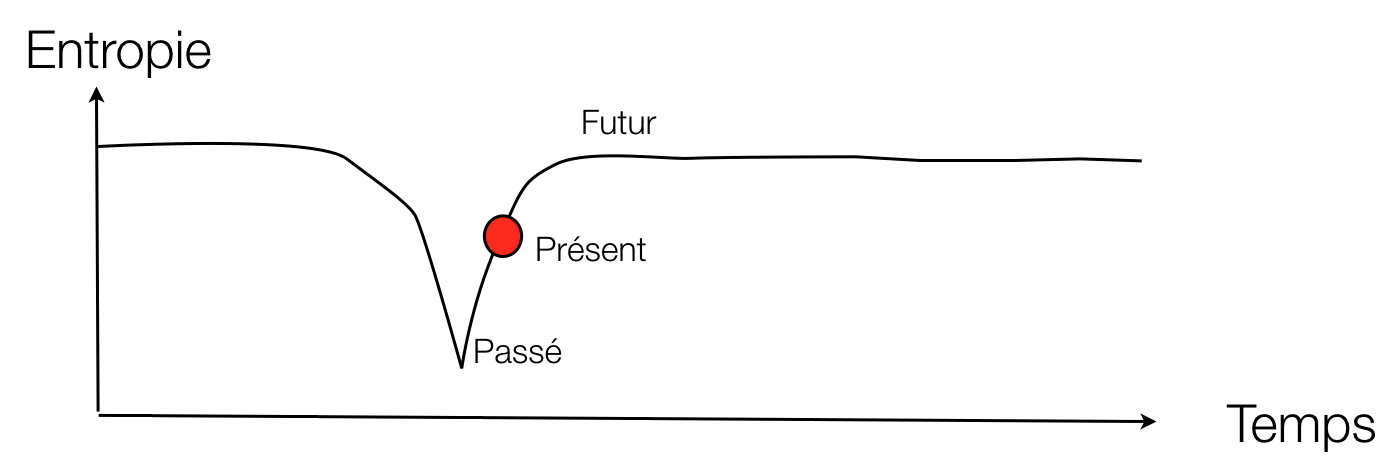
\includegraphics[height=5cm]{figs/fluctuation.png}
	\caption[fluctuation d'entropie]{La possibilité d'une fluctuation d'entropie pour expliquer le démarrage de notre Univers. Passé et futur correspondent aux époques où l'entropie était respectivement basse et haute~: le Big-Bang serait le résultat d'une fluctuation d'entropie sur une situation globale où cette entropie est constante.}
	\label{f:fluctuation}
\end{figure}

Ce scénario a des implications profondes. Dans un premier temps, le point de départ de l'évolution de notre Univers est par définition le Big Bang\index{Big-Bang} : l'instant où cette fluctuation opère correspond donc au début de cette évolution et le Big Bang trouve son origine dans une fluctuation statistique. Par ailleurs, ce scénario suggère que nous sommes dans une phase anormale, précédée et suivie par des états d'équilibres stables qui correspondent aux vrais états naturels de notre Univers : la physique à l'oeuvre autour de nous ne serait que la manifestation d'un retour à la normale durant une phase transitoire.

\newthought{Malheureusement ce scénario souffre d'un paradoxe}. A titre d'exemple, rappelons la définition de l'entropie $S$ dans le cas micro-canonique\index{micro-canonique} :
\begin{equation}
S=k_B\log{\Omega},
\end{equation}
où $\Omega$ désigne le nombre de configurations accessibles pour un état macroscopique donné. Le nombre de configurations correspondant à une valeur d'entropie donnée est :
\begin{equation}
\Omega=e^{S/k_B}.
\end{equation}
Par conséquent, toute fluctuation sur l'entropie est démultipliée exponentiellement et si on compare 2 fluctuations d'entropie d'amplitudes différentes, elles conduisent à des nombres de configurations qui sont \textit{exponentiellement} différentes: 2 états microscopiques d'entropies légèrement différentes peuvent correspondre à 2 états de probabilités qui n'ont rien à voir\sidenote{on comprend aisément qu'un macro-état à grand nombre de configurations est plus probable qu'un autre à moins de configurations disponibles}. Une fluctuation d'entropie profonde est donc particulièrement difficile à produire et toute fluctuation d'amplitude intermédiaire est bien plus aisée à mettre en place : l'amplitude de la fluctuation nécessaire à l'évolution constatée autour de nous est de fait quasi-impossible à générer. Souvent on illustre cette difficulté par le \textit{paradoxe des cerveaux de Boltzmann}\index{entropie!cerveaux de Boltzmann} : il est possible que l'Univers tel que nous l'observons soit le fruit d'une sensation ressentie par un cerveau flottant dans le cosmos. Soit un Univers chaotique, rempli de particules~: il est bien plus probable que ces particules s'arrangent brièvement sous la forme de ce cerveau avec ses propres sensations plutôt qu'elles s'organisent par  hasard de façon à créer les conditions qui vont être amenée à créer des étoiles, avec des planètes qui hébergent la vie, vie qui va produire une intelligence en mesure d'étudier le cosmos... Rationnellement, ce cerveau flottant a bien plus de chances refléter la réalité du monde que le second scénario. Bien sûr, cette conclusion est insupportable et de fait probablement fausse mais elle est inévitable si l'évolution de l'Univers constatée est le fruit d'une fluctuation statistique.

Pour conclure, nous n'avons pas actuellement d'explication simple et satisfaisante quand à la faible valeur initiale de l'entropie cosmique et par extension pour la mise en route de notre Univers en train d'évoluer. Des mécanismes exotiques sont néanmoins proposés, sans validation observationnelles à ce jour~: par exemple, notre Univers est peut-être en communication avec d'autres Univers\sidenote{on parle aussi de \textit{multivers}}, permettant au nôtre d'avoir une entropie faible en augmentant celles des autres cosmos\sidenote{à la manière de réservoirs de gaz en communication}. Ou bien il s'agit simplement d'un tirage favorable des paramètres de notre cosmos, dont une valeur initiale de l'entropie faible~: rappelons que cela fait de notre Univers un monde imparfait, obligé d'évoluer, là où un monde 'parfait' pourrait rester statique du fait de sa perfection initiale.  Cet Univers aurait des temps caractéristiques d'évolution très longs, durant lesquels rien n'évolue, rien ne se passe ou presque. Et rappelons également qu'une entropie élevée, parfaite, correspond aux configurations les plus nombreuses, les plus probables: nous l'avons échappé belle.